\documentclass[a4paper]{article}

\usepackage[utf8]{inputenc}
\usepackage[spanish,es-tabla]{babel}
\usepackage[T1]{fontenc}
\usepackage{microtype}
\usepackage{newspaper}
\usepackage{multicol}
\usepackage{multirow}
\usepackage{array}
\usepackage{url}
\usepackage{hyperref}
\usepackage[table]{xcolor}
\hypersetup{
	%% colores de enlaces
	colorlinks,
	linkcolor={red!50!black},
	citecolor={blue!50!black},
	urlcolor={blue!80!black},
	%% metadata del PDF generado
	%% estos metadatos se deben actualizar con cada edición
  pdftitle={Gaceta Galénica - V01N02},
	pdfsubject={Boletín científico del Servicio de Urgencias de la Policlínica Lic. Manuel María Valdés},
	pdfauthor={Moisés Serrano Samudio},
	pdfkeywords={
		Carlos Finlay,
		dengue,
		malaria,
		Canal de Panamá}
}

%% ============================================================================
%% Referencias
%% ============================================================================
\usepackage{csquotes}
\usepackage[
	backend=biber,
	style=nejm,
  minnames=3,
  maxnames=5,
  articledoi=false,
]{biblatex}

%% Hace que las referencias aparezcan como superíndices
\let\cite=\supercite

%% Añade el documento con referencias bibtex
\addbibresource{referencias.bib}

%% Reduce el tamaño de fuente de las referencias
\renewcommand*{\bibfont}{\scriptsize}

%% ============================================================================
%% Box para viñetas
%% ============================================================================
\usepackage[many]{tcolorbox}
\newtcolorbox{boxClinica}{
	sharpish corners, % better drop shadow
	boxrule = 0pt,
	toprule = 1.5pt, % top rule weight
	enhanced,
	%% {xshift}{yshift}{offset}{step}{options}
	fuzzy shadow = {0pt}{-2pt}{-0.5pt}{0.5pt}{black!35}
}

%% ============================================================================
%% Imágenes
%% ============================================================================
\usepackage{float}
\usepackage{graphicx}
\usepackage{wrapfig}
\usepackage{caption}
\captionsetup[figure]{font=footnotesize}

%% ============================================================================
%% Cabecera
%% ============================================================================
\date{\today}
\currentvolume{0}
\currentissue{0}
\SetPaperName{Gaceta Galénica}
\SetHeaderName{Gaceta Galénica}
\SetPaperLocation{Ciudad de Panamá}
\SetPaperSlogan{''\textit{Ciencia, Verdad, Academia}''}
\SetPaperPrice{SU-PMMV}

\newcommand{\NewsAuthor}[1]{%
	\hfill Por \textsc{#1} \vspace{4pt}
	\par \normalfont
}

%%
\usepackage{newspaper-mod}
%%
\renewcommand{\headlinestyle}{\itshape\Large\lsstyle}
% \renewcommand{\bylinestyle}{\bfseries\Large\raggedright}
%%

%%%%%%%%%  Front matter   %%%%%%%%%%


\begin{document}

\maketitle

\begin{multicols}{3}


\byline{Editorial}{Moisés Serrano Samudio}

La construcción del Canal de Panamá fue uno de los grandes logros de la
ingeniería en los albores del siglo XX, pero esta no fue posible hasta lograr
controlar las enfermedades tropicales que azotaron a los franceses y los
trabajadores que trajeron para el fallido intento de replicar el éxito
del Canal de Suéz.

La malaria y la fiebre amarilla son patologías que tienen en común la
transmisión por vectores, los llamados zancudos o mosquitos cuyas hembras
hematófagas arrinconaron a la empresa del Conde De Lesseps dando la estocada
mortal que agravó años de malos manejos y acusaciones de corrupción y
malversación de fondos.

La historia suele darle mayor reconocimiento al Coronel William C. Gorgas por
el logro en la erradicación de la fiebre amarilla y disminución en la
incidencia de malaria en las Ciudades de Panamá y Colón. Para lograr esta
hazaña tuvo que pararse en hombros de un gigante poco reconocido, el
cubano Carlos Finlay de quien recorreremos algo de su biografía.

Lo invitamos a usted, querido lector a que honre nuestras páginas
producto de una revisión histórica exhaustiva sobre estas dos enfermedades
tropicales que aún a día de hoy siguen presentes en nuestro medio.

\closearticle


\headline{¿Quién fue Carlos Juan Finlay?}

Médico y científico cubano. Nace en 1833 en Puerto Príncipe, Capitanía
General de Cuba, cuando aún Cuba pertenecía al Imperio Español\cite{biojcf}.

\begin{wrapfigure}{L}{0.18\textwidth}
	\begin{center}
		\vspace{-10pt}
		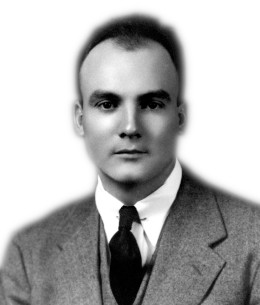
\includegraphics[width=0.17\textwidth]{trdawber.jpg}
	\end{center}
	\caption*{Dr. Carlos Juan Finlay}
\end{wrapfigure}

texto

\closearticle


\headline{Malaria y Fiebre Amarilla. Una revisión histórica}

texto

\begin{boxClinica}

Paciente masculino de 64 años es traído al servicio de urgencias por personal
de prehospitalaria por síncope con previa historia de palpitaciones, mareos,
debilidad y diaforesis. Sus signos vitales son: PA 160/106 mmHg, FC 141 lpm,
FR 21 cpm, SpO2 92\%, peso 125 kg, estatura 1,65 m. Tiene como antecedentes
importantes tabaquismo y dislipidemia. Se encuentra desorientado y disneico.

\end{boxClinica}

texto

\end{multicols}

\closearticle

\begin{multicols}{3}

\printbibliography[heading=none]

\end{multicols}


\end{document}
